---
id: tkz-euclide-ejemplo-04
title: Puntos
description: "Define y representa puntos etiquetados en el plano."
keywords: [puntos, etiquetas, plano]
tags: [tkzDefPoint,tkzDrawPoints,tkzLabelPoints]
sort: 4
---
\documentclass[tikz,border=2mm]{standalone}
\usepackage{tkz-euclide}

\begin{document}
    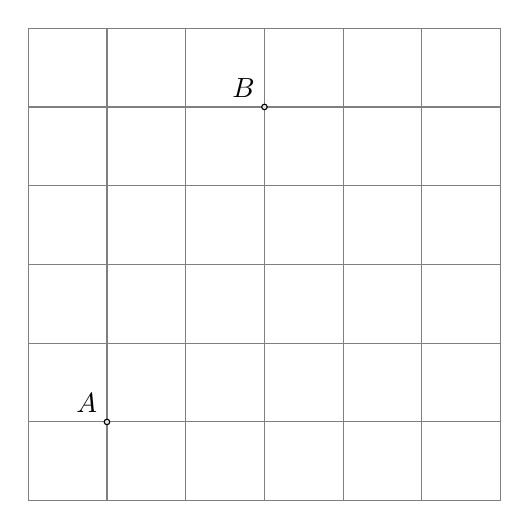
\begin{tikzpicture}
        % Define el sistema de coordenadas ortogonales.
        \tkzInit[xmin=0,xmax=6,ymin=0,ymax=6]
        % Dibuja los ejes x,y
        \tkzDrawXY
        % Dibuja una cuadrícula en el área definida.
        \tkzGrid
    
        % Define puntos individuales: A,B.
        \tkzDefPoint(1,1){A}
        \tkzDefPoint(3,5){B}
    
        % Dibuja los puntos definidos.
        \tkzDrawPoints(A,B)
    
        % Etiqueta los puntos arriba a la izquierda.
        \tkzLabelPoints[above left](A,B)
    \end{tikzpicture}
\end{document}